\chapter{Project Planning}

\section{Planned Phases of the Project}
The project is divided into several phases, which must be completed in sequence. Throughout these phases, the interim and final reports will be developed concurrently as a skeleton.
\begin{enumerate}
	\item Research - This phase consists of finding and reading existing literature. It is at this time that the project idea is developed fully.
	\item Simple Implementation - In this phase, a proof of concept implementation will be developed. It will entail a simple swarm learning algorithm learning on a basic dataset, without any complex problems. This implementation will be build upon in further phases.
	\item Interim Report - This phase is focussed on filling out and finalising the interim report.
	\item Main development - In this phase, the iterative development of the swarm learning algorithm will occur. This is actually a repetition of four sub-phases:
	\begin{enumerate}
		\item Further research on real-world problem
		\item Implement real-world problem and test current solution
		\item Implement mitigations and test / evaluate
		\item Document any discoveries and evaluations of mitigations
	\end{enumerate}
	\item Final report - In this phase, the final report will be written up.
	\item Housekeeping - This is the final phase which is used for any extra jobs that were not able to be completed in other phases.
\end{enumerate}



\section{Completed Work}
A Gantt chart was created to plan the completion of different sections of the project prior to the interim stage. This chart was closely followed and proved to be a valuable tool for time management. The Gantt chart was developed after the initial project brief was submitted.

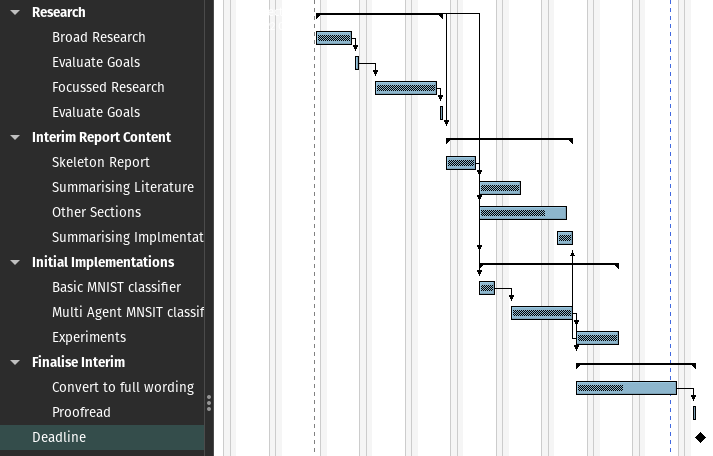
\includegraphics[width=\textwidth]{gantt_pre}


\section{Remaining Work}
A second Gantt chart was created to plan the project after the interim stage. This chart was developed near the end of the first semester, after a more thorough understanding of the project had been obtained through research. The chart only includes plans for two problems, as it was determined that this is the minimum number required for the scope of the project. If the problems are completed more quickly than anticipated, additional problems will be incorporated into the development phase. A large block of time has been allocated in the housekeeping phase to act as a buffer in case any other aspect of the project takes longer than expected. The ideal outcome is for the project to be submitted at the beginning of this period.

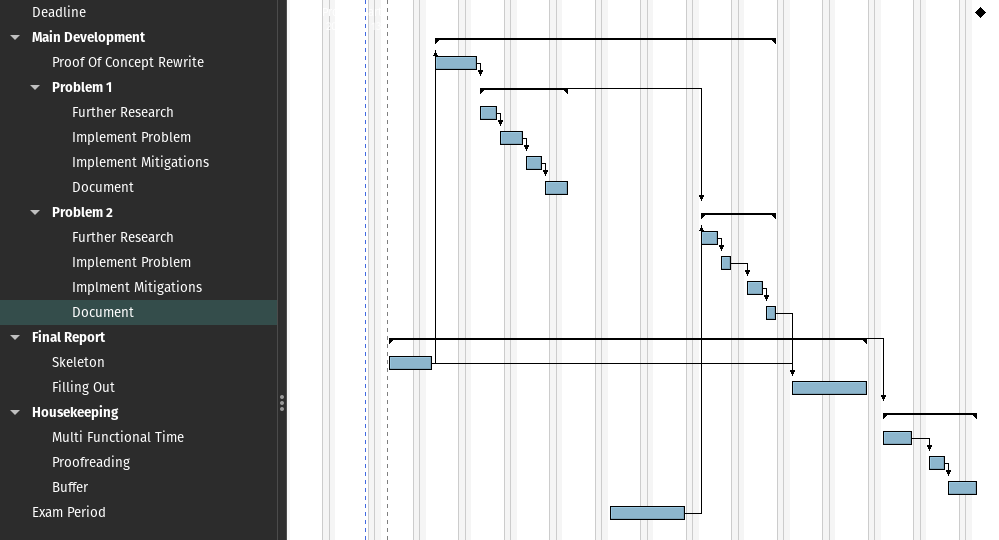
\includegraphics[width=\textwidth]{gantt_post}



\section{Risk Assessment}
\subsection{Personal Issues}

\subsubsection{Description}
This risk entails all personal issues which cause the author to be unable to do work, such as illness.

\subsubsection{Risk Calculations}
\emph{Severity (1-5):} 3 \\
\emph{Likelihood (1-5):} 3 \\
\emph{Overall Risk (1-25):} \textbf{9}

\subsubsection{Mitigation}
As much as possible, the codebase will be designed such that individual sections and modules have minimal dependencies on other sections. This means that, even if the author is unable to work for a period of time, some less critical sections can be omitted without significantly impacting the rest of the project.

\subsection{Hardware Failure - Local Computer}
\subsubsection{Description}
This risk entails a failure on the authors local computer of any kind, such as a graphics card or storage breakage.

\subsubsection{Risk Calculations}
\emph{Severity (1-5):} 4 \\
\emph{Likelihood (1-5):} 2 \\
\emph{Overall Risk (1-25):} \textbf{8}

\subsubsection{Mitigation}
To mitigate storage based failures, the project will be regularly backed up to GitHub. If a core component of the work computer breaks, the author has access to a personal laptop and the Zepler Labs. The deep learning environment along with dependencies is backed up to the authors Google Drive in the form of a docker image, so that switching to a new computer would be a smooth process.

\subsection{Algorithm Fails to Work}
\subsubsection{Description}
This risk describes a situation where the algorithm of swarm learning does not function as well as expected. However, this is very unlikely as swarm learning has been proven to work in numerous papers CITE ME.

\subsubsection{Risk Calculations}
\emph{Severity (1-5):} 5 \\
\emph{Likelihood (1-5):} 1 \\
\emph{Overall Risk (1-25):} \textbf{5}

\subsubsection{Mitigation}
This is not an ideal situation, nevertheless it may be possible to shift the project away from swarm learning and onto federated learning. Federated learning is more commonly used and therefore has more literature, meaning that it is more likely to be an achievable goal to implement it. This would be a last resort though.